\documentclass[letter,11pt]{article}

\usepackage[spanish,es-nodecimaldot]{babel}
\usepackage[utf8]{inputenc}

\usepackage{lmodern}
\usepackage[T1]{fontenc}
\usepackage{textcomp}

\usepackage{framed}
\usepackage[svgnames]{xcolor}
\colorlet{shadecolor}{Gainsboro!50}

\usepackage[labelfont=bf]{caption}
\usepackage{graphicx}
\usepackage{pstricks}

\usepackage{anysize}
\marginsize{3cm}{2cm}{2cm}{3cm}

\usepackage{siunitx}
\usepackage{amsmath}
\usepackage{array}
\usepackage{csquotes}
\usepackage{steinmetz}
\usepackage{stmaryrd}

\usepackage{fancyhdr}
\usepackage{lastpage}
\pagestyle{fancy}
\fancyhf{}
\fancyhead[LE,RO]{Laboratorio de Circuitos Eléctricos III}
\fancyfoot[CO,CE]{\thepage\ de \pageref{LastPage}}

\special{papersize=215.9mm,279.4mm}

\usepackage[
    pdfauthor={Carlos Eduardo Caballero Burgoa},%
    pdftitle={Laboratorio de Circuitos Eléctricos III},%
    pdfsubject={Medida de la potencia activa y reactiva trifásica en circuitos
    con carga desequilibrada},%
    colorlinks,%
    citecolor=black,%
    filecolor=black,%
    linkcolor=black,%
    urlcolor=black,
    breaklinks]{hyperref}
\usepackage{breakurl}

\renewcommand{\arraystretch}{1.2}

\begin{document}

\begin{titlepage}
    \begin{center}
        {\Large UNIVERSIDAD MAYOR DE SAN SIMÓN}\\
        \vspace*{0.15cm}
        {\large FACULTAD DE CIENCIAS Y TECNOLOGÍA}\\
        \vspace*{0.10cm}
        DEPARTAMENTO DE ELÉCTRICA-ELECTRÓNICA\\
        \vspace*{3.0cm}
        {\Large \textbf{LABORATORIO DE CIRCUITOS ELÉCTRICOS III}}\\
        \vspace*{0.3cm}
        {\Large \textbf{INFORME No. 6}}\\
        \vspace*{3.5cm}
        {\Large \textbf{MEDIDA DE LA POTENCIA ACTIVA Y REACTIVA\\
        TRIFÁSICA EN CIRCUITOS CON CARGA DESEQUILIBRADA}}\\
    \end{center}

    \vspace*{5.3cm}
    \leftskip=7.95cm
    \noindent
    \textbf{Estudiante:}\\
    Caballero Burgoa, Carlos Eduardo.\\
    \newline
    \textbf{Carrera:}\\
    Ing. Electromecánica.\\
    \newline
    \textbf{Docente:}\\
    Ing. Marco Antonio Vallejo Camacho.\\
    \newline
    \textbf{Grupo:} 2F (Martes).\\
\textbf{Fecha de entrega:} 29 de Octubre del 2024.\\
\end{titlepage}

\section{Cálculos teóricos}

\begin{figure}[!h]
\centering
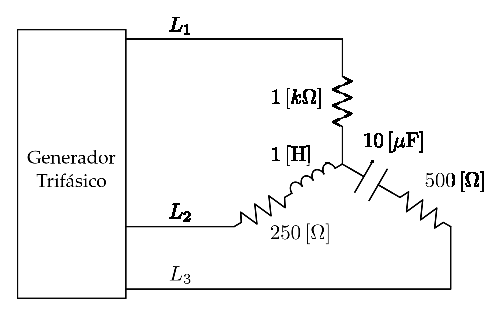
\includegraphics[scale=0.95]{figura1.eps}
\caption{Circuito trifásico desequilibrado con carga estrella.}
\label{circuito1}
\end{figure}

Considerando un circuito trifásico con carga estrella desequilibrado
(\textbf{Figura~\ref{circuito1}}) con las siguientes cargas de fase:

\begin{itemize}
    \item \textbf{Carga 1}: $R_1=1[k\Omega]$.
    \item \textbf{Carga 2}: $R_2=250[\Omega]$ y $L=1[H]$.
    \item \textbf{Carga 3}: $R_3=500[\Omega]$ y $C=10[\mu F]$.
\end{itemize}

Con voltajes de linea $U_L=380[\text{V}]$ y con frecuencia de $50[\text{Hz}]$,
se hallan las corrientes de fase y linea para hallar las potencias activa y
reactiva:

Se calcula la frecuencia angular ($\omega$):
\begin{equation*}
    \begin{split}
        \omega&=2\pi f\\
              &=2\pi(50)\\
              &=100\pi[\text{rad}/\text{s}]\\
    \end{split}
\end{equation*}

Se hallan las impedancias en el dominio de frecuencia:
\begin{equation*}
    \begin{split}
        Z_1 &= R_1\\
            &= 1000[\Omega]\\
        Z_2 &= R_2+j\omega L\\
            &= 250+j100\pi[\Omega]\\
        Z_3 &= R_3+\frac{1}{j\omega C}\\
            &= 500-j\frac{1000}{\pi}[\Omega]\\
    \end{split}
\end{equation*}

Considerando una secuencia positiva:
\begin{equation*}
    \begin{split}
        U_a &= 220\phase{0^{\circ}}\,[\text{V}]\\
        U_b &= 220\phase{-120^{\circ}}\,[\text{V}]\\
        U_c &= 220\phase{120^{\circ}}\,[\text{V}]\\
    \end{split}
\end{equation*}

Se calcula el voltaje entre neutros con el teorema de \emph{Millman}:
\begin{equation*}
    \begin{split}
        U_0 &= \dfrac{
                   \dfrac{U_a}{Z_1}+\dfrac{U_b}{Z_2}+\dfrac{U_c}{Z_3}
               }{
                   \dfrac{1}{Z_1}+\dfrac{1}{Z_2}+\dfrac{1}{Z_3}
               }\\
            &= \dfrac{
                   \dfrac{220\phase{0^{\circ}}}{1000}+
                   \dfrac{220\phase{-120^{\circ}}}{250+j100\pi}+
                   \dfrac{120\phase{120^{\circ}}}{500-j(1000/\pi)}
               }{
                   \dfrac{1}{1000}+
                   \dfrac{1}{250+j100\pi}+
                   \dfrac{1}{500-j(1000/\pi)}
               }\\
            &= 159.99\phase{-173.20^{\circ}}[\text{V}]\\
    \end{split}
\end{equation*}

A partir del voltaje de neutro se calculan las corrientes de linea:
\begin{equation*}
    \begin{split}
        I_{L_1} &= \frac{U_a - U_0}{Z_1}\\
                &= \frac{200\phase{0^{\circ}}
                   -159.99\phase{-173.20^{\circ}}}{500}\\
                &= 0.38\phase{2.86^{\circ}}[\text{A}]\\
        I_{L_2} &= \frac{U_b - U_0}{Z_2}\\
                &= \frac{200\phase{-120^{\circ}}
                   -159.99\phase{-173.20^{\circ}}}{250+j100\pi}\\
                &= 0.44\phase{-125.59^{\circ}}[\text{A}]\\
        I_{L_3} &= \frac{U_c - U_0}{Z_3}\\
                &= \frac{200\phase{120^{\circ}}
                   -159.99\phase{-173.20^{\circ}}}{500-j(1000/\pi)}\\
                &= 0.36\phase{109.35^{\circ}}[\text{A}]\\
    \end{split}
\end{equation*}

La potencia activa en cada impedancia y el total es:
\begin{equation*}
    \begin{split}
        P_{Z_1} &= |I_{L_1}|^2\,(\Re\{Z_1\})\\
                &= 0.38^2\,(1000)\\
                &= 143.90[\text{W}]\\
        P_{Z_2} &= |I_{L_2}|^2\,(\Re\{Z_2\})\\
                &= 0.44^2\,(250)\\
                &= 49.361[\text{W}]\\
        P_{Z_3} &= |I_{L_3}|^2\,(\Re\{Z_3\})\\
                &= 0.36^2\,(500)\\
                &= 65.845[\text{W}]\\
        P_T &= P_{Z_1} + P_{Z_2} + P_{Z_3}\\
            &= 143.90 + 49.361 + 65.845\\
            &= 259.102[\text{W}]\\
    \end{split}
\end{equation*}

La potencia reactiva en cada impedancia y el total es:
\begin{equation*}
    \begin{split}
        Q_{Z_1} &= |I_{L_1}|^2\,(\Im\{Z_1\})\\
                &= 0.38^2\,(0)\\
                &= 0[\text{VAR}]\\
        Q_{Z_2} &= |I_{L_2}|^2\,(\Im\{Z_2\})\\
                &= 0.44^2\,(314.161)\\
                &= 62.029[\text{VAR}]\\
        Q_{Z_3} &= |I_{L_3}|^2\,(\Im\{Z_3\})\\
                &= 0.36^2\,(-318.31)\\
                &= -41.918[\text{VAR}]\\
        Q_T &= Q_{Z_1} + Q_{Z_2} + Q_{Z_3}\\
            &= 0 + 62.029 - 41.918\\
            &= 20.111[\text{VAR}]\\
    \end{split}
\end{equation*}

La potencia total calculada por el método de los dos vatímetros es:
\begin{equation*}
    \begin{split}
        P_{W_1} &= U_{L_1 L_3}\,I_{L_1}^*\\
                &= (380\phase{-30^{\circ}})(0.38\phase{-2.86^{\circ}})^*\\
                &= 121.080 - j78.219[\text{VA}]\\
        P_{W_2} &= U_{L_2 L_3}\,I_{L_2}^*\\
                &= (380\phase{-90^{\circ}})(0.44\phase{-125.59^{\circ}})^*\\
                &= 137.307 + j98.274[\text{VA}]\\
        P_T &= \Re\{P_{W_1}\} + \Re\{P_{W_2}\}\\
            &= 121.080 + 137.307\\
            &= 258.388[\text{W}]\\
        Q_T &= \Im\{P_{W_1}\} + \Im\{P_{W_2}\}\\
            &= -78.219 + 98.274\\
            &= 20.0555[\text{VAR}]\\
    \end{split}
\end{equation*}

\subsection{Resumen de resultados}
En la siguiente tabla se resumen los valores obtenidos teóricamente:

\begin{center}
    \begin{tabular}{|c||c|c|c|c||c|}
    \hline
    & \textbf{$Z_1$} & $Z_2$ & $Z_3$ & \textbf{Total} & \textbf{Vatímetros}
    \tabularnewline \hline \hline
    $P$ &
    $143.90[\text{W}]$ &
    $49.361[\text{W}]$ &
    $65.845[\text{W}]$ &
    $259.102[\text{W}]$ &
    $258.388[\text{W}]$
    \tabularnewline \hline
    $Q$ &
    $0[\text{VAR}]$ &
    $62.029[\text{VAR}]$ &
    $-41.918[\text{VAR}]$ &
    $20.111[\text{VAR}]$ &
    $20.0555[\text{VAR}]$
    \tabularnewline \hline
    \end{tabular}
\end{center}

\section{Simulación}
Se utilizó el software \emph{Electronic Workbench v5.12.} para simular
el circuito, la carga en estrella puede verse en la
\textbf{Figura~\ref{simulacion1}}:

\begin{figure}[!h]
\centering
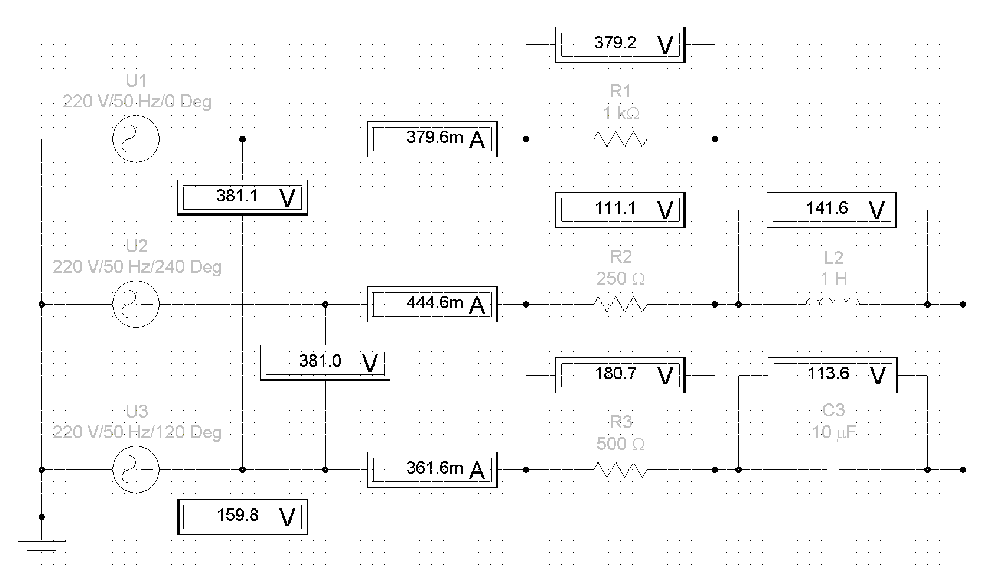
\includegraphics[scale=1.00]{simulacion/practica6.1.eps}
\caption{Simulación del circuito desequilibrado con carga estrella.}
\label{simulacion1}
\end{figure}

\subsection{Resumen de resultados}
En la siguiente tabla se resumen los valores obtenidos de la simulación: 

\begin{center}
    \begin{tabular}{|c||c|c|c|}
    \hline
    & \textbf{$Z_1$} & $Z_2$ & $Z_3$
    \tabularnewline \hline \hline
    $I_Z$ &
    $379.6[m\text{A}]$ &
    $444.6[m\text{A}]$ &
    $361.6[m\text{A}]$
    \tabularnewline \hline
    $U_R$ &
    $379.2[\text{V}]$ &
    $111.1[\text{V}]$ &
    $180.7[\text{V}]$
    \tabularnewline \hline
    $U_X$ &
    $0[\text{V}]$ &
    $141.6[\text{V}]$ &
    $113.6[\text{V}]$
    \tabularnewline \hline
    $P=U_R\,I_Z$ &
    $143.944[\text{W}]$ &
    $49.395[\text{W}]$ &
    $65.341[\text{W}]$
    \tabularnewline \hline
    $Q=U_X\,I_Z$ &
    $0[\text{VAR}]$ &
    $62.9554[\text{VAR}]$ &
    $(-)41.0778[\text{VAR}]$
    \tabularnewline \hline
    $P_T$ &
    \multicolumn{3}{|c|}{$258.68[\text{W}]$}
    \tabularnewline \hline
    $Q_T$ &
    \multicolumn{3}{|c|}{$21.878[\text{VAR}]$}
    \tabularnewline \hline
    \end{tabular}
\end{center}

\section{Tablas y mediciones}
Se presentan los resultados obtenidos con las mediciones realizadas en 
laboratorio y el calculo de las potencias activa y reactiva a partir del voltaje
y corriente:

\begin{center}
    \begin{tabular}{|c||c|c|c|}
    \hline
    & \textbf{$Z_1$} & $Z_2$ & $Z_3$
    \tabularnewline \hline \hline
    $I_Z$ &
    $0.36[\text{A}]$ &
    $0.42[\text{A}]$ &
    $0.34[\text{A}]$
    \tabularnewline \hline \hline
    $U_R$ &
    $381[\text{V}]$ &
    $106[\text{V}]$ &
    $184[\text{V}]$
    \tabularnewline \hline
    $U_X$ &
    $0[\text{V}]$ &
    $134[\text{V}]$ &
    $110[\text{V}]$
    \tabularnewline \hline \hline
    $P=U_R\,I_Z$ &
    $137.16[\text{W}]$ &
    $44.52[\text{W}]$ &
    $62.56[\text{W}]$
    \tabularnewline \hline
    $Q=U_X\,I_Z$ &
    $0[\text{VAR}]$ &
    $56.28[\text{VAR}]$ &
    $(-)37.4[\text{VAR}]$
    \tabularnewline \hline \hline
    $P_T$ &
    \multicolumn{3}{|c|}{$244.24[\text{W}]$}
    \tabularnewline \hline
    $Q_T$ &
    \multicolumn{3}{|c|}{$18.88[\text{VAR}]$}
    \tabularnewline \hline
    \end{tabular}
\end{center}

Se presentan los resultados obtenidos con las mediciones realizadas con el
método de los dos vatímetros para el calculo de potencia:

\begin{center}
    \begin{tabular}{|c||c|c|}
    \hline
    $W_1$ & $123[\text{W}]$
    \tabularnewline \hline
    $W_2$ & $136[\text{W}]$
    \tabularnewline \hline \hline
    $Q_1$ & $-74[\text{VAR}]$
    \tabularnewline \hline
    $Q_2$ & $94[\text{VAR}]$
    \tabularnewline \hline \hline
    $P_T$ & $259[\text{W}]$
    \tabularnewline \hline
    $Q_T$ & $20[\text{VAR}]$
    \tabularnewline \hline
    \end{tabular}
\end{center}

\section{Cuestionario}

\begin{enumerate}

\item \textbf{Compare la potencia total obtenida por cada método tanto en la
activa como en la reactiva. ¿Cual de las dos formas se aproxima mejor al
resultado teórico? ¿Es la misma situación que un circuito equilibrado?}

Las potencias activa y reactiva calculadas son:

\begin{center}
    \begin{tabular}{|c|c||c|}
    \hline
    \textbf{Teórico ($U{\times}I$)} & \textbf{Activa} & $259.102[\text{W}]$
    \tabularnewline \hline
                                    & \textbf{Reactiva} & $20.111[\text{VAR}]$
    \tabularnewline \hline \hline
    \textbf{Teórico (Dos vatímetros)} & \textbf{Activa} & $258.388[\text{W}]$
    \tabularnewline \hline
                                      & \textbf{Reactiva} & $20.0555[\text{VAR}]$
    \tabularnewline \hline \hline
    \textbf{Simulado ($U{\times}I$)} & \textbf{Activa} & $258.68[\text{W}]$
    \tabularnewline \hline
                                     & \textbf{Reactiva} & $21.878[\text{VAR}]$
    \tabularnewline \hline \hline
    \textbf{Laboratorio ($U{\times}I$)} & \textbf{Activa} & $244.24[\text{W}]$
    \tabularnewline \hline
                                        & \textbf{Reactiva} & $18.88[\text{VAR}]$
    \tabularnewline \hline \hline
    \textbf{Laboratorio (Dos vatímetros)} & \textbf{Activa} & $259[\text{W}]$
    \tabularnewline \hline
                                          & \textbf{Reactiva} & $20[\text{VAR}]$
    \tabularnewline \hline
    \end{tabular}
\end{center}

Existen diferencias pequeñas entre los valores obtenidos, los valores más
cercanos a los valores teóricos son: los calculados a partir de los dos
vatímetros. Esto difiere del caso del circuito equilibrado, donde las mediciones
del producto del voltaje y la corriente fueron mas próximas a los valores
teóricos.

\item \textbf{Que pasaría si la secuencia fuera negativa, ¿la potencia activa o
reactiva total cambiaría o no? Haga sus cálculos para esta secuencia para
justificar su respuesta.}

Considerando una secuencia negativa:
\begin{equation*}
    \begin{split}
        U_a &= 220\phase{0^{\circ}}\,[\text{V}]\\
        U_b &= 220\phase{120^{\circ}}\,[\text{V}]\\
        U_c &= 220\phase{-120^{\circ}}\,[\text{V}]\\
    \end{split}
\end{equation*}

Se calcula el voltaje entre neutros con el teorema de \emph{Millman}:
\begin{equation*}
    \begin{split}
        U_0 &= \dfrac{
                   \dfrac{U_a}{Z_1}+\dfrac{U_b}{Z_2}+\dfrac{U_c}{Z_3}
               }{
                   \dfrac{1}{Z_1}+\dfrac{1}{Z_2}+\dfrac{1}{Z_3}
               }\\
            &= \dfrac{
                   \dfrac{220\phase{0^{\circ}}}{1000}+
                   \dfrac{220\phase{120^{\circ}}}{250+j100\pi}+
                   \dfrac{120\phase{-120^{\circ}}}{500-j(1000/\pi)}
               }{
                   \dfrac{1}{1000}+
                   \dfrac{1}{250+j100\pi}+
                   \dfrac{1}{500-j(1000/\pi)}
               }\\
            &= 111.57\phase{32.36^{\circ}}[\text{V}]\\
    \end{split}
\end{equation*}

A partir del voltaje de neutro se calculan las corrientes de linea:
\begin{equation*}
    \begin{split}
        I_{L_1} &= \frac{U_a - U_0}{Z_1}\\
                &= \frac{200\phase{0^{\circ}}
                   -111.57\phase{32.36^{\circ}}}{500}\\
                &= 0.14\phase{-25.40^{\circ}}[\text{A}]\\
        I_{L_2} &= \frac{U_b - U_0}{Z_2}\\
                &= \frac{200\phase{120^{\circ}}
                   -111.57\phase{32.36^{\circ}}}{250+j100\pi}\\
                &= 0.60\phase{95.87^{\circ}}[\text{A}]\\
        I_{L_3} &= \frac{U_c - U_0}{Z_3}\\
                &= \frac{200\phase{-120^{\circ}}
                   -111.57\phase{32.36^{\circ}}}{500-j(1000/\pi)}\\
                &= 0.54\phase{-96.74^{\circ}}[\text{A}]\\
    \end{split}
\end{equation*}

La potencia activa en cada impedancia y el total es:
\begin{equation*}
    \begin{split}
        P_{Z_1} &= |I_{L_1}|^2\,(\Re\{Z_1\})\\
                &= 0.14^2\,(1000)\\
                &= 19.382[\text{W}]\\
    \end{split}
\end{equation*}
\begin{equation*}
    \begin{split}
        P_{Z_2} &= |I_{L_2}|^2\,(\Re\{Z_2\})\\
                &= 0.60^2\,(250)\\
                &= 91.230[\text{W}]\\
        P_{Z_3} &= |I_{L_3}|^2\,(\Re\{Z_3\})\\
                &= 0.54^2\,(500)\\
                &= 148.49[\text{W}]\\
        P_T &= P_{Z_1} + P_{Z_2} + P_{Z_3}\\
            &= 19.382 + 91.230 + 148.49\\
            &= 259.102[\text{W}]\\
    \end{split}
\end{equation*}

La potencia reactiva en cada impedancia y el total es:
\begin{equation*}
    \begin{split}
        Q_{Z_1} &= |I_{L_1}|^2\,(\Im\{Z_1\})\\
                &= 0.14^2\,(0)\\
                &= 0[\text{VAR}]\\
        Q_{Z_2} &= |I_{L_2}|^2\,(\Im\{Z_2\})\\
                &= 0.60^2\,(314.161)\\
                &= 114.64[\text{VAR}]\\
        Q_{Z_3} &= |I_{L_3}|^2\,(\Im\{Z_3\})\\
                &= 0.54^2\,(-318.31)\\
                &= -94.532[\text{VAR}]\\
        Q_T &= Q_{Z_1} + Q_{Z_2} + Q_{Z_3}\\
            &= 0 + 114.64 - 94.532\\
            &= 20.111[\text{VAR}]\\
    \end{split}
\end{equation*}

La potencia total calculada por el método de los dos vatímetros es:
\begin{equation*}
    \begin{split}
        P_{W_1} &= U_{L_1 L_3}\,I_{L_1}^*\\
                &= (380\phase{30^{\circ}})(0.14\phase{-25.40^{\circ}})^*\\
                &= 30.040 + j43.548[\text{VA}]\\
        P_{W_2} &= U_{L_2 L_3}\,I_{L_2}^*\\
                &= (380\phase{90^{\circ}})(0.60\phase{95.87^{\circ}})^*\\
                &= 228.347 - j23.492[\text{VA}]\\
        P_T &= \Re\{P_{W_1}\} + \Re\{P_{W_2}\}\\
            &= 30.040 + 228.347\\
            &= 258.388[\text{W}]\\
        Q_T &= \Im\{P_{W_1}\} + \Im\{P_{W_2}\}\\
            &= 43.548 - 23.492\\
            &= 20.0555[\text{VAR}]\\
    \end{split}
\end{equation*}

Los valores de potencia activa y reactiva para ambas secuencias se resumen en la
siguiente tabla:

\begin{center}
    \begin{tabular}{|c|c||c|c|c|c||c|}
    \hline
    & & \textbf{$Z_1$} & $Z_2$ & $Z_3$ & \textbf{Total} & \textbf{Vatímetros}
    \tabularnewline \hline \hline
    $(+)$ &
    $P[\text{W}]$ &
    $143.90$ &
    $49.361$ &
    $65.845$ &
    $259.102$ &
    $258.388$
    \tabularnewline \hline
    & $Q[\text{VAR}]$ &
    $0$ &
    $62.029$ &
    $-41.918$ &
    $20.111$ &
    $20.0555$
    \tabularnewline \hline \hline
    $(-)$ &
    $P[\text{W}]$ &
    $19.382$ &
    $91.230$ &
    $149.49$ &
    $259.102$ &
    $258.388$
    \tabularnewline \hline
    & $Q[\text{VAR}]$ &
    $0$ &
    $114.64$ &
    $-94.532$ &
    $20.111$ &
    $20.0555$
    \tabularnewline \hline
    \end{tabular}
\end{center}

Los valores de potencia en cada impedancia varían, pero los valores totales de
la carga estrella no varían según la secuencia.

\item \textbf{Demuestre analíticamente que el método de los dos vatímetros nos
da la potencia trifásica total en el caso de un circuito desequilibrado.}

Los valores tomados por los vatímetros según la definición de potencia son:

\begin{equation*}
    \begin{split}
        W_1 &= \Re\{\bar{U}_{ac}\,\bar{I}_{a}^*\}\\
        W_2 &= \Re\{\bar{U}_{bc}\,\bar{I}_{b}^*\}\\
    \end{split}
\end{equation*}

\begin{figure}[!h]
\centering
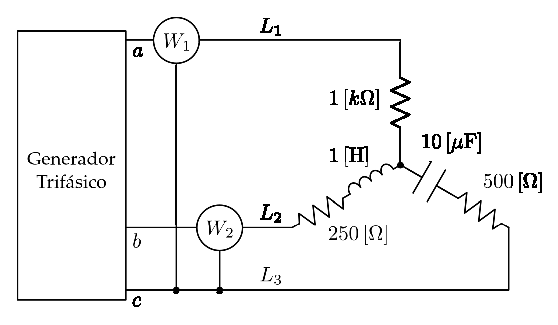
\includegraphics[scale=0.95]{figura2.eps}
\caption{Medición de potencia con dos vatímetros.}
\label{circuito2}
\end{figure}

Por tanto:
\begin{equation*}
    \begin{split}
        W_1 + W_2 &= \Re\{\bar{U}_{ac}\,\bar{I}_{a}^*\}+
                     \Re\{\bar{U}_{bc}\,\bar{I}_{b}^*\}\\
                  &= \Re\{\bar{U}_{ac}\,\bar{I}_{a}^*+
                          \bar{U}_{bc}\,\bar{I}_{b}^*\}\\
                  &= \Re\{(\bar{U}_a+\bar{U}_c)\,\bar{I}_a^*+
                          (\bar{U}_b+\bar{U}_c)\,\bar{I}_b^*\}\\
                  &= \Re\{\bar{U}_a\,\bar{I}_a^*+
                          \bar{U}_c\,\bar{I}_a^*+
                          \bar{U}_b\,\bar{I}_b^*+
                          \bar{U}_c\,\bar{I}_b^*\}\\
                  &= \Re\{\bar{U}_a\,\bar{I}_a^*+
                          \bar{U}_b\,\bar{I}_b^*+
                          \bar{U}_c\,(\bar{I}_a^*+\bar{I}_b^*)\}\\
                  &= \Re\{\bar{U}_a\,\bar{I}_a^*+
                          \bar{U}_b\,\bar{I}_b^*+
                          \bar{U}_c\,\bar{I}_c^*\}\\
                  &= \Re\{\bar{U}_a\,\bar{I}_a^*\}+
                     \Re\{\bar{U}_b\,\bar{I}_b^*\}+
                     \Re\{\bar{U}_c\,\bar{I}_c^*\}\\
                  &= P_{W_1} + P_{W_2} + P_{W_3}\\
                  &= P_T\\
    \end{split}
\end{equation*}

\end{enumerate}

\section{Conclusiones y Recomendaciones}
Se calcularon, simularon y demostraron experimentalmente las medición de la
potencia con los métodos de la suma de potencias individuales, y el método de
los dos vatímetros sobre una carga estrella desequilibrada, y fueron
verificadas en todos los casos.

También se verifico que la potencia total en un circuito trifásico no varia
dependiendo de la secuencia del generador.

\end{document}

